\documentclass[letterpaper,10pt]{article}
\usepackage{graphicx}
\usepackage{listings}
\usepackage{fullpage}
\usepackage{fixltx2e}
\usepackage{multirow}
\usepackage{amssymb,amsmath}
\usepackage{mathtools}
\usepackage[hyperfootnotes=false]{hyperref}
\usepackage{url}
\usepackage{subfig}
\usepackage{relsize}
\usepackage{enumitem}
\usepackage{fancyhdr}
\setlength{\headheight}{14pt}
\pagestyle{fancy}
\headsep = 20pt

% Lineskip mods
\linespread{1.0}
\setlength{\parskip}{0.5\baselineskip}
\setlength{\parindent}{0pt}
\newlength\docparskip
\parskip=6pt
\setlength{\docparskip}{\parskip}
\renewcommand{\arraystretch}{1.085}
\usepackage{xcolor}
\lstset{basicstyle=\ttfamily,
  showstringspaces=false,
  commentstyle=\color{red},
  keywordstyle=\color{blue}
}
\begin{document}

\fancyhf{}
\fancyhead[L]{AME 60614: Numerical Methods}
\fancyhead[R]{YourName: Problem Set 0}
\fancyfoot[C]{\thepage}

\thispagestyle{plain}
\begin{center}
  \large
  \textbf{AME 60614: Numerical Methods} \\
  \textbf{Fall 2021} \\
  \vspace{0.5em}
  \textbf{Problem Set 0} \\
  \vspace{1em}
  Your Name Here!
\end{center}

\vspace{1.5em}


\section{Code Documentation}

\begin{enumerate}
\item Download the document \texttt{sample\_ps0.tex} and \texttt{sample\_figure.eps} from the course Sakai page. Rename the file \texttt{lastname\_firstname\_ps0.tex}, and edit the report to add your name. Compile it using \texttt{pdflatex} or the \LaTeX\ editor of your choice.
  
\item Document your response to Problem 2 in your report. Use appropriately highlighted code listings for codes requested in Problem 2. Print a copy and bring it to class on the due date.
\end{enumerate}

Here is an example of how to insert a figure with \texttt{includegraphics\{\}}. In general, figures should be at the top of a page. However, in this case, the title is at the top, so we specify explicitly to put the figure here using ``[h]''. You can refer to the figure by its label: Figure~\ref{fig:grid}.
\begin{figure}[h]
  \centering
  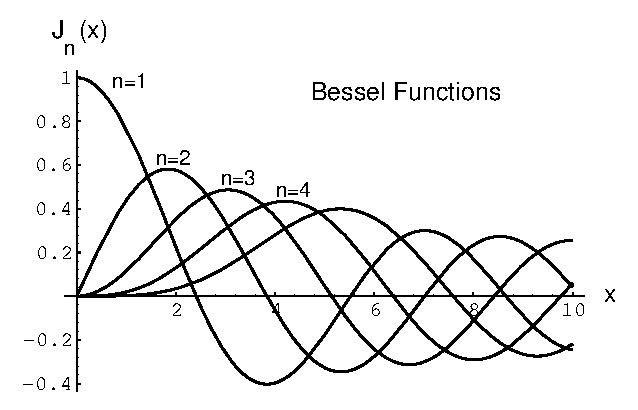
\includegraphics[width=0.4\textwidth]{sample_figure.eps}
  \caption{Sample figure showing Bessel functions.}
  \label{fig:grid}
\end{figure}
  

\section{Computing in Parallel}


The Mandelbrot set is defined as the collection of points $c=(x,iy)$ on $\Omega=[-2,0.5]\times[-2i,2i]\subset\mathbb{C}$ for which the iterative sequence
\begin{equation*}
  z_{n+1}(c) =z_n^2(c) + c
\end{equation*}
remains bounded, where $z_n(c) \in\Omega$ is the value of the sequence at a point $c$ for iteration $n$, $n\in[0,\infty)$, and $z_0=0$.

It may be shown that the sequence becomes unbounded if
\begin{equation*}
  |z_n(c)| > 2
\end{equation*}
for any $n$. To determine if a point is a member of the Mandelbrot set, one must check each point in the domain under the infinite sequence and exclude those points for which $|z_n(c)|>2$. In practice, this involves creating a grid of finite resolution and iterating on each point a maximum of \texttt{MAX\_ITER} times.


The following is an example code listing. Modify it to include your source code for solving the Mandelbrot set. Do not forget the other items requested in the problem set document.
{\small\begin{lstlisting}[language=c,frame=single]
#include <stdio.h>
#include <stdlib.h>

int main() {

  // Define an integer counter
  int counter = 0;
  counter = 0;

  // Allocate double-precision data on the heap
  //   Note: *data denotes a pointer to memory
  int N = 10;
  double *data = malloc(N*sizeof(double));

  // Loop to perform operations
  for (int i=0; i<N; i++) {
    data[i] = 2.5*i;
    printf("Hello world %d %4.3f\n", counter, data[i]);
    counter++; 
  }

  // Read the saved data in reverse
  for (int i=N; i>0; i--) {
    printf("%d %4.3f\n", i, data[i-1]);
  }

  // Clean up
  free(data);
  data = NULL;
  
  return 0;
}
\end{lstlisting}}





\end{document}
